\documentclass{beamer}
\usepackage[latin1]{inputenc}
\usetheme{Frankfurt}

\title{Programming Exercises}
\subtitle{Project Presentation}   
\institute{Frankfurt University of Applied Sciences}
\author{Marcus Vinicius Pereira Araujo 1106149\\Purit Thong-On 1106398\\Piyaphat Russamitinakornkul 1106291} 
\date{July 23, 2015} 
\logo{
\includegraphics[height=1cm]{icon.png}}


\begin{document}

	\begin{frame}
		\titlepage
	\end{frame} 
	
	\begin{frame}
		\frametitle{Table of contents}
		\tableofcontents
	\end{frame}
	 
	

	\section{UVa Online Judge} 
		\begin{frame}
			\sectionpage
		\end{frame}

		\begin{frame}
			\frametitle{UVa Online Judge}
			Group Members:\\
			\begin{enumerate}
				\item Marcus Vinicius Pereira Araujo
				\item Purit Thong-On
				\item Piyaphat Russamitinakornkul
			\end{enumerate} 
		\end{frame}

		\subsection{Marcus' UVa Online Judge}
			\begin{frame}
				\subsectionpage
			\end{frame}

			\begin{frame}
				\frametitle{UVa Online Judge - Marcus}
				\begin{center}
					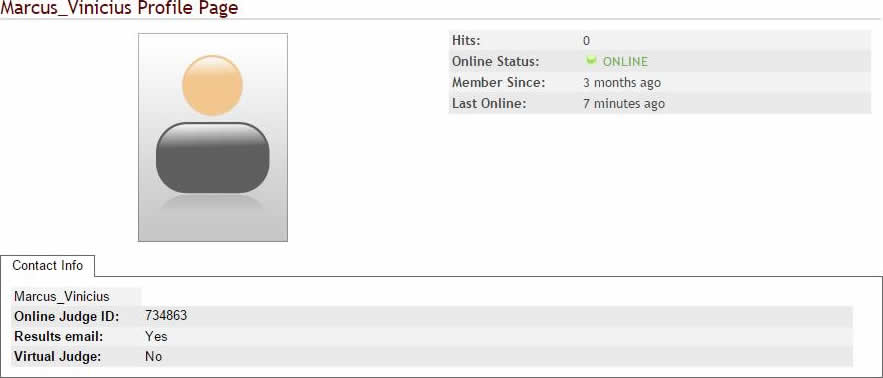
\includegraphics[scale=0.35]{Profile2} 
				\end{center}
			\end{frame}

			\begin{frame}
				\frametitle{UVa Online Judge - Marcus}
				\begin{center}
					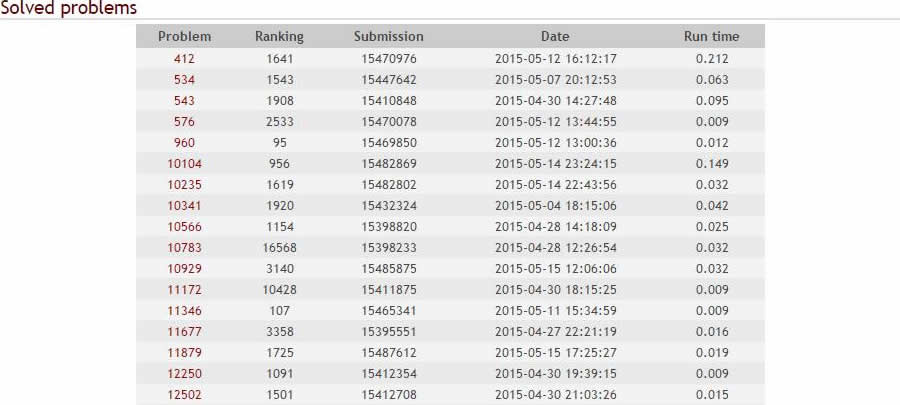
\includegraphics[scale=0.38]{Solved2} 
				\end{center}
			\end{frame}

			\begin{frame}
				\frametitle{UVa Online Judge - Marcus}
				\begin{center}
					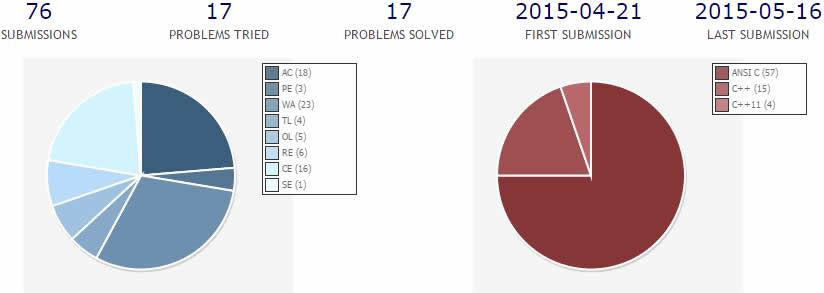
\includegraphics[scale=0.38]{Statistics2} 
				\end{center}
			\end{frame}

			\begin{frame}
				\frametitle{UVa Online Judge - Marcus}
				\begin{center}
					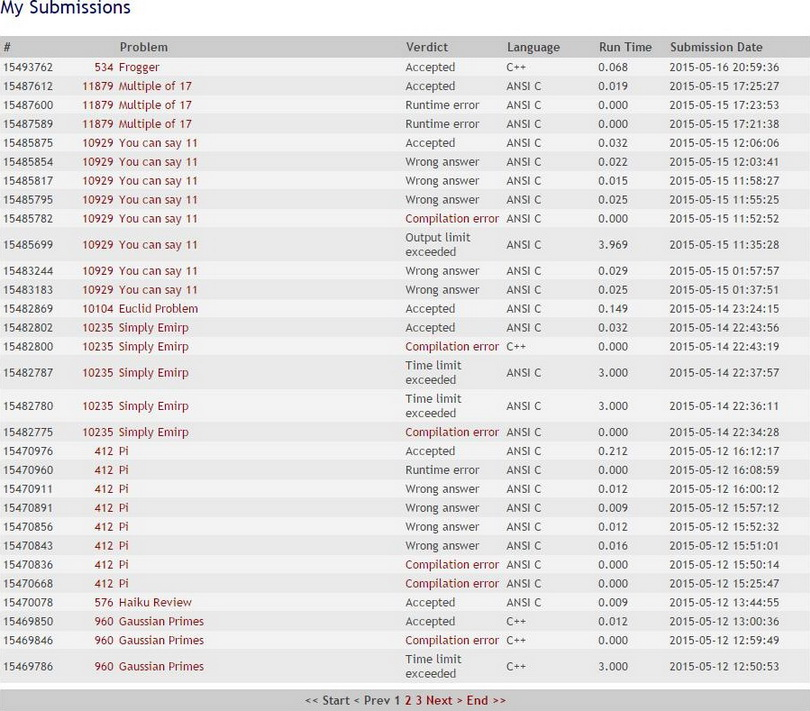
\includegraphics[scale=0.30]{Submission2-1} 
				\end{center}
			\end{frame}

			\begin{frame}
				\frametitle{UVa Online Judge - Marcus}
				\begin{center}
					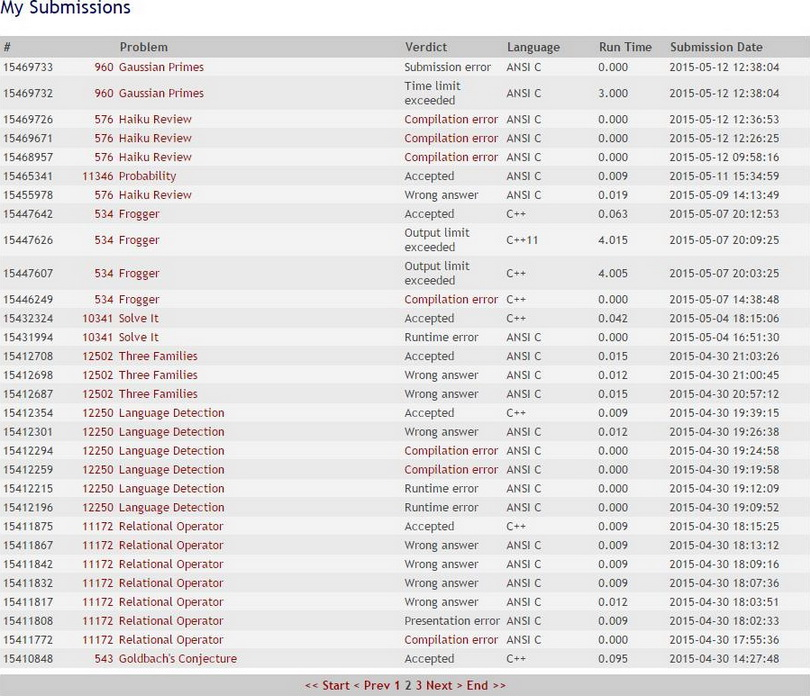
\includegraphics[scale=0.30]{Submission2-2} 
				\end{center}
			\end{frame}

			\begin{frame}
				\frametitle{UVa Online Judge - Marcus}
				\begin{center}
					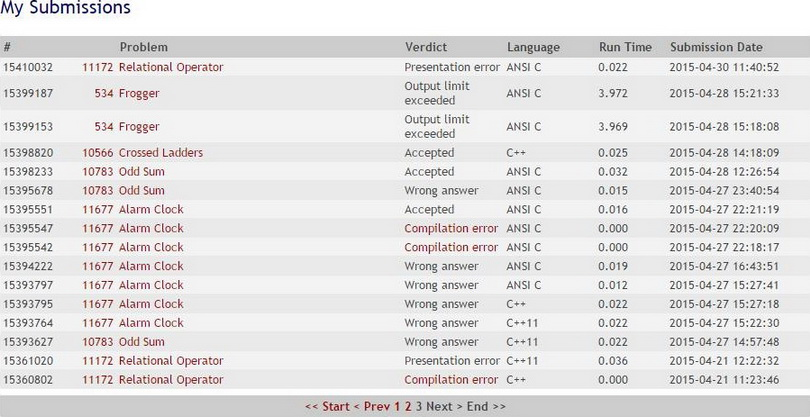
\includegraphics[scale=0.35]{Submission2-3} 
				\end{center}
			\end{frame}

		\subsection{Purit's UVa Online Judge}
			\begin{frame}
				\subsectionpage
			\end{frame}

			\begin{frame}
				\frametitle{UVa Online Judge - Purit}
				\begin{center}
					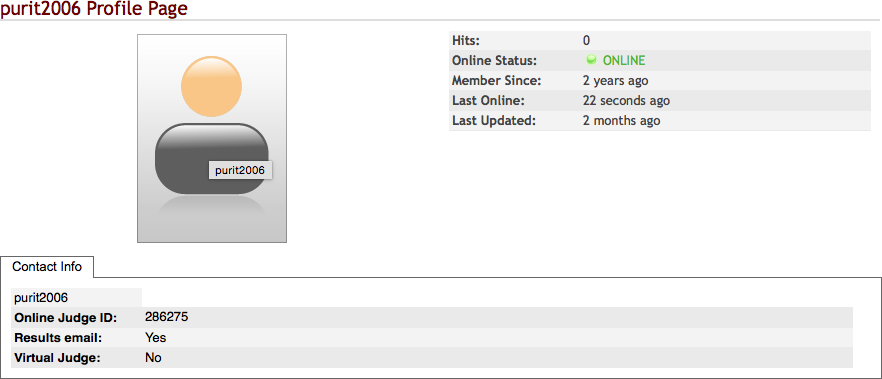
\includegraphics[scale=0.36]{Profile3} 
				\end{center}
			\end{frame}

			\begin{frame}
				\frametitle{UVa Online Judge - Purit}
				\begin{center}
					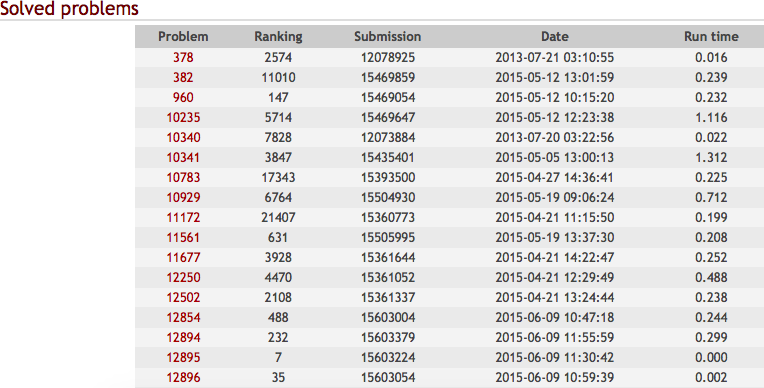
\includegraphics[scale=0.38]{Solved3} 
				\end{center}
			\end{frame}

			\begin{frame}
				\frametitle{UVa Online Judge - Purit}
				\begin{center}
					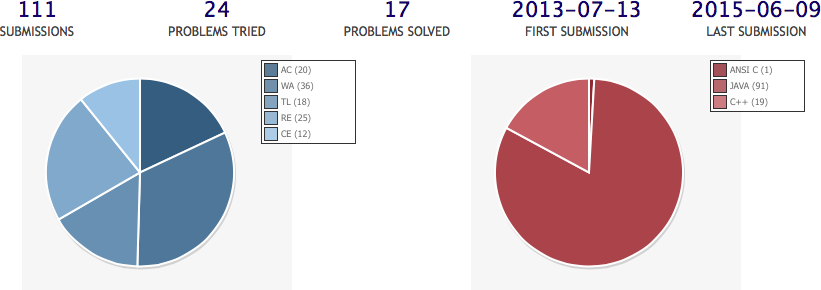
\includegraphics[scale=0.38]{Statistics3} 
				\end{center}
			\end{frame}

			\begin{frame}
				\frametitle{UVa Online Judge - Purit}
				\begin{center}
					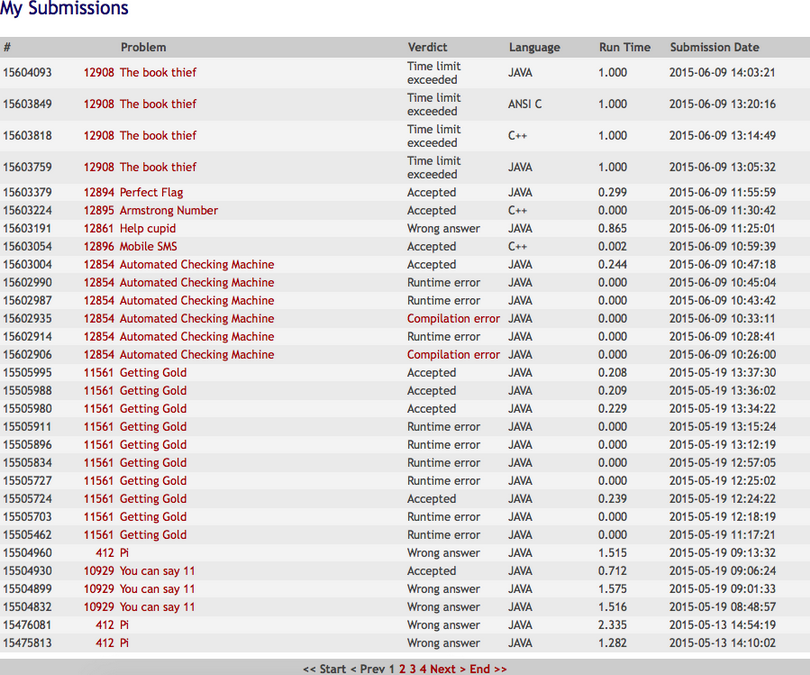
\includegraphics[scale=0.30]{Submission3-1} 
				\end{center}
			\end{frame}

			\begin{frame}
				\frametitle{UVa Online Judge - Purit}
				\begin{center}
					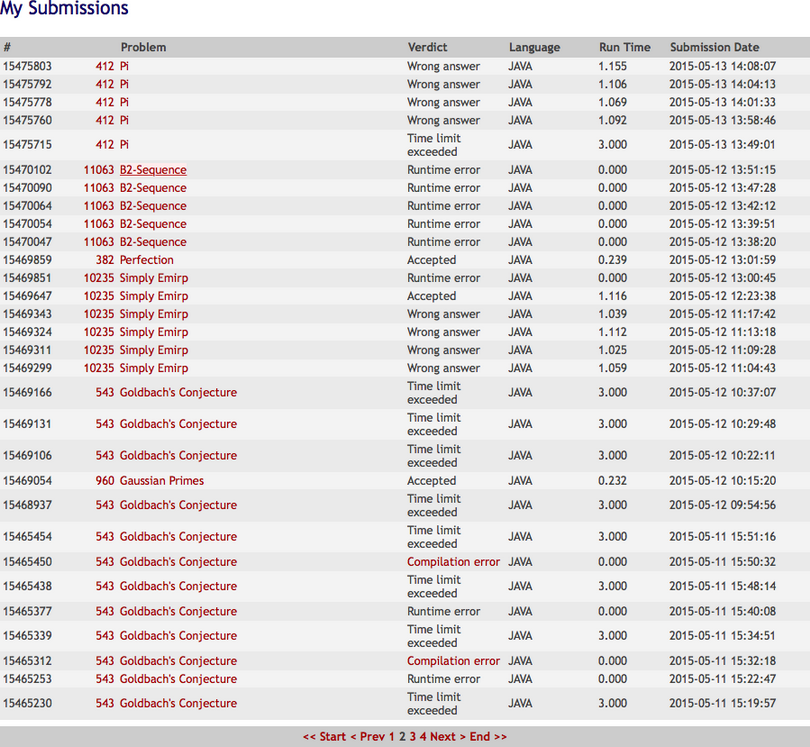
\includegraphics[scale=0.27]{Submission3-2} 
				\end{center}
			\end{frame}

			\begin{frame}
				\frametitle{UVa Online Judge - Purit}
				\begin{center}
					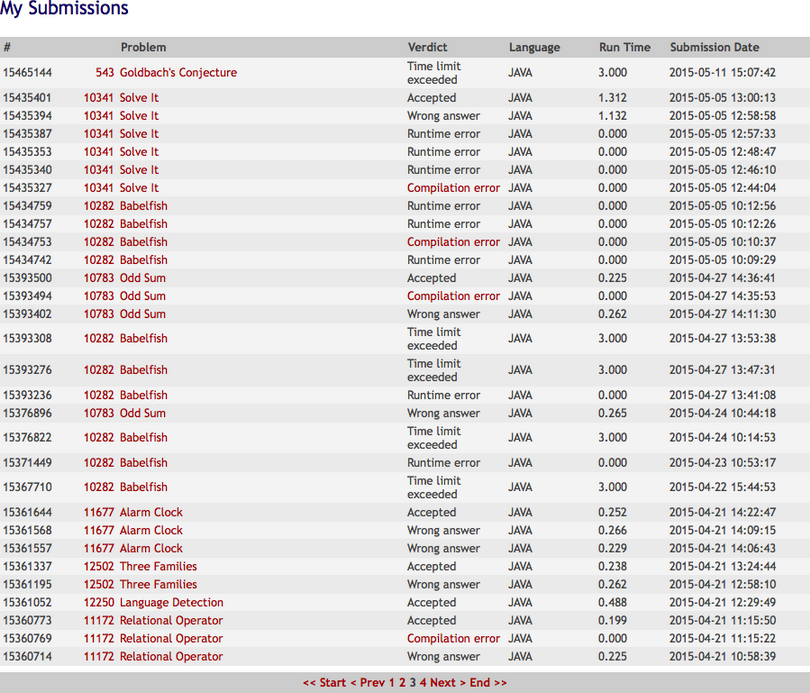
\includegraphics[scale=0.30]{Submission3-3} 
				\end{center}
			\end{frame}

			\begin{frame}
				\frametitle{UVa Online Judge - Purit}
				\begin{center}
					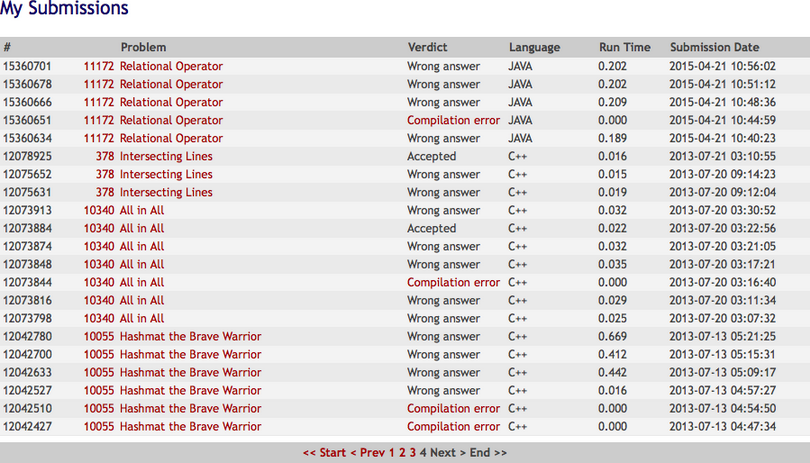
\includegraphics[scale=0.4]{Submission3-4} 
				\end{center}
			\end{frame}

		\subsection{Piyaphat's UVa Online Judge}
			\begin{frame}
				\subsectionpage
			\end{frame}

			\begin{frame}
				\frametitle{UVa Online Judge - Piyaphat}
				\begin{center}
					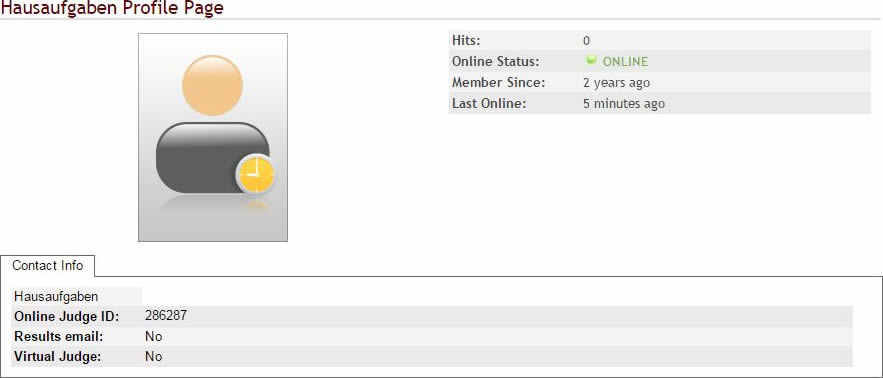
\includegraphics[scale=0.48]{Profile1} 
				\end{center}
			\end{frame}

			\begin{frame}
				\frametitle{UVa Online Judge - Piyaphat}
				\begin{center}
					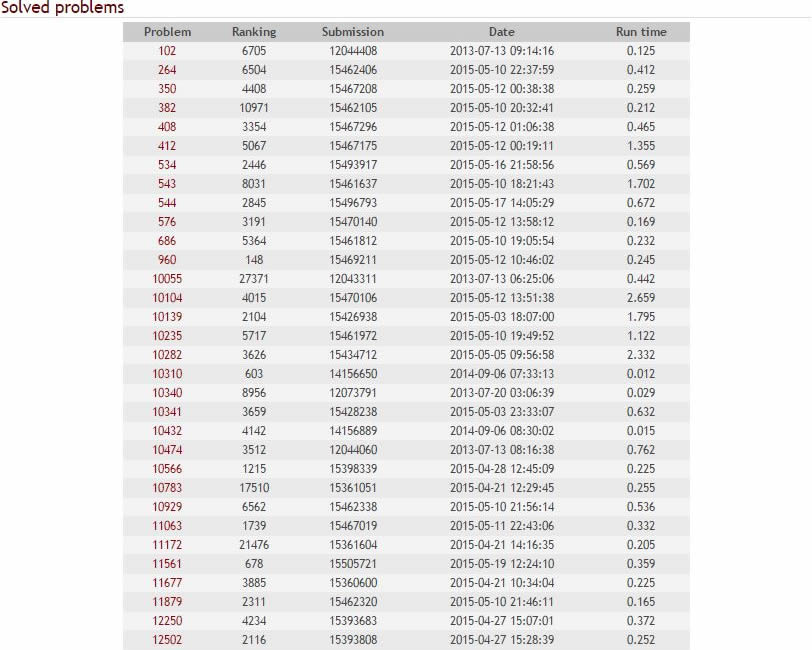
\includegraphics[scale=0.4]{Solved1} 
				\end{center}
			\end{frame}

			\begin{frame}
				\frametitle{UVa Online Judge - Piyaphat}
				\begin{center}
					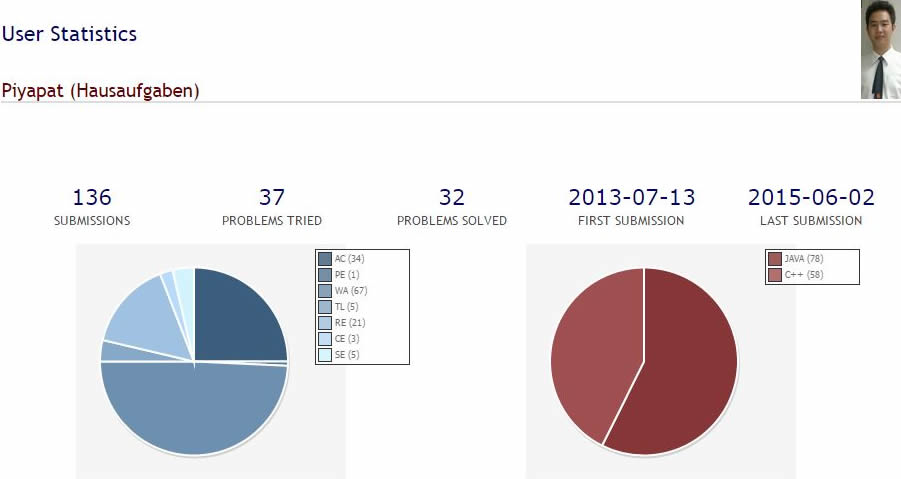
\includegraphics[scale=0.4]{Statistics1} 
				\end{center}
			\end{frame}

			\begin{frame}
				\frametitle{UVa Online Judge - Piyaphat}
				\begin{center}
					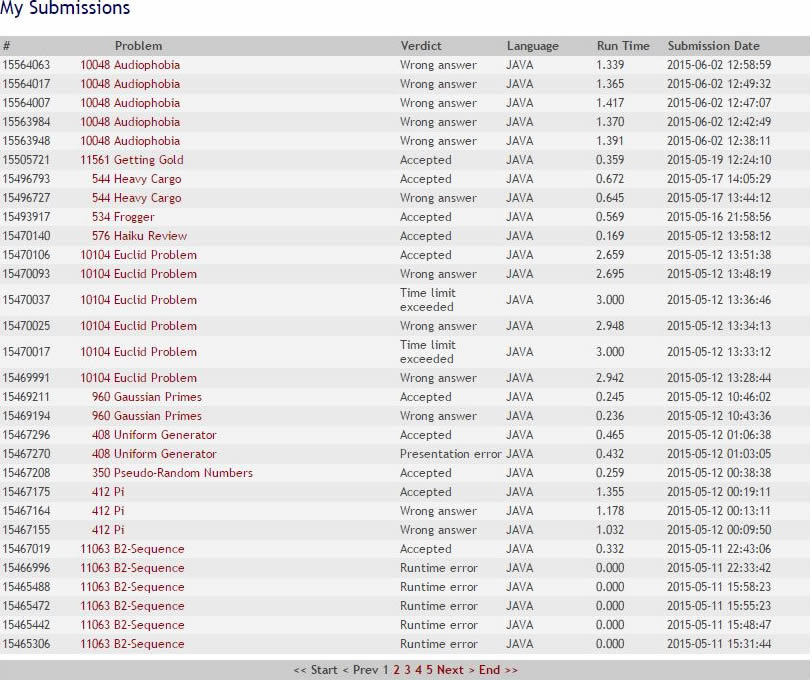
\includegraphics[scale=0.4]{Submission1-1} 
				\end{center}
			\end{frame}

			\begin{frame}
				\frametitle{UVa Online Judge - Piyaphat}
				\begin{center}
					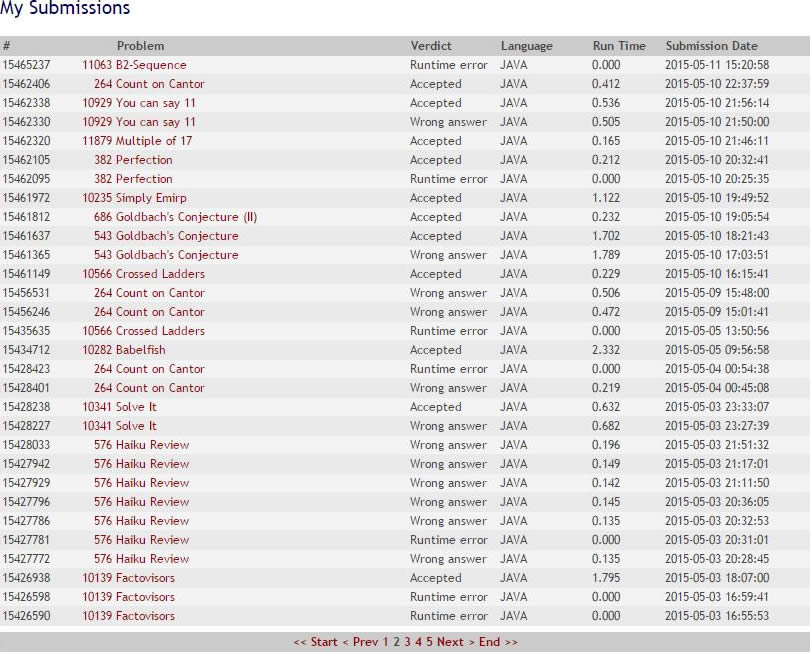
\includegraphics[scale=0.4]{Submission1-2} 
				\end{center}
			\end{frame}

			\begin{frame}
				\frametitle{UVa Online Judge - Piyaphat}
				\begin{center}
					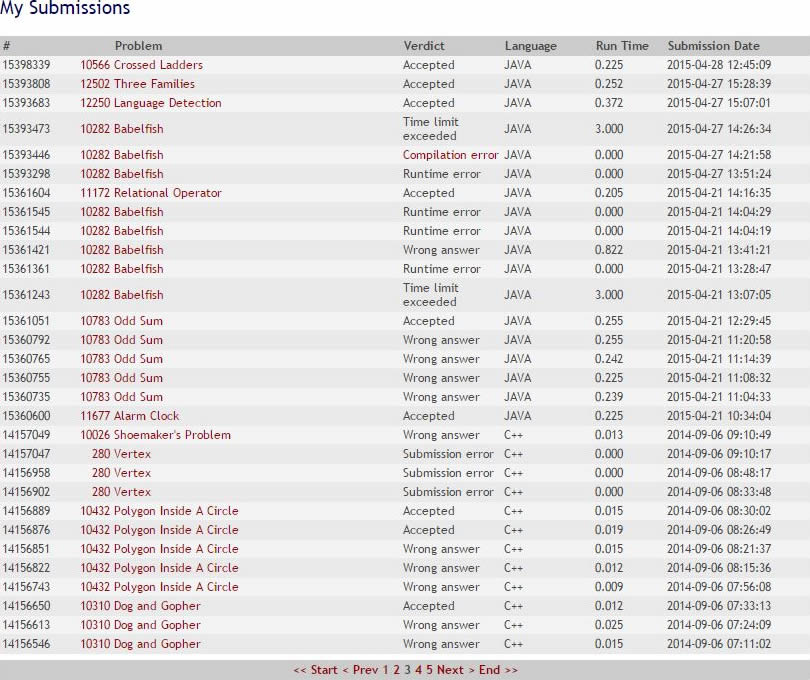
\includegraphics[scale=0.4]{Submission1-3} 
				\end{center}
			\end{frame}

			\subsection{Programming Day}
			\begin{frame}
				\frametitle{UVa Online Judge - Programming Day}
				Solved Problems:\\
				\begin{table}
					\begin{tabular}{c | l}
						Question No. & Question Name \\
						\hline
						12854 & Automated Checking Machine\\
						12894 & Perfecct Flag\\
						12896 & Mobile SMS
					\end{tabular}
				\caption{Solved Programming Day Problems}
				\end{table}
			\end{frame}



	\section{Kakuro Solver} 
		\begin{frame}
			\sectionpage
		\end{frame}

		\subsection{Project Requirement}
			\begin{frame}
				\frametitle{Kakuro Problem Requirement}
				Requirement:\\
				\hspace{1cm}Create a program to generate and solve Kakuro problems using "Genetic Algorithms".
			\end{frame}

		\subsection{Problem Description}
			\begin{frame}
				\frametitle{Kakuro Solver Problem Description}
				Problem:
				\begin{itemize} [<+->]
					\item How to generate an effective Kakuro Puzzle?
					\item How to validate a Kakuro Puzzle?
					\item How to solve any given valid Kakuro Puzzle?
				\end{itemize} 
			\end{frame}
	
		\subsection{Genetic Algorithms}
			\begin{frame}
				\frametitle{Genetic Algorithms - Initialization}
				\begin{itemize} [<+->]
					\item Initialization $\rightarrow$ Create a {\it population}.
					\item A {\it population} consists of an {\it individual}.
					\item Each {\it individual} is a possible solution to solve the puzzle.\\It is not necessary that the {\it individual} has to be a final solution.
				\end{itemize} 
			\end{frame}

			\begin{frame}
				\frametitle{Genetic Algorithms - Evaluation}
				\begin{itemize} [<+->]
					\item Evaluation $\rightarrow$ Determine {\it fitness} value. Each {\it individual} has its own {\it fitness} value.
					\item An {\it individual's fitness value} will determine the similarity to the ideal solution.
				\end{itemize} 
			\end{frame}

			\begin{frame}
				\frametitle{Genetic Algorithms on Kakuro}
				\begin{columns}[c]
					\column{6cm}
					\begin{itemize}
						\item Each puzzle cells has a set a corresponding cells for filling solutions.\\
						\begin{center}
							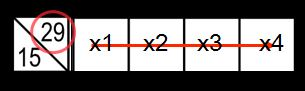
\includegraphics[scale=0.4]{kakuroExample} 
						\end{center}
						\item Difference between the average of the values filled in the cells and its corresponding puzzle value.
						\item The {\it fitness} value for an ideal solution is "0.0"
					\end{itemize}

					\column{6cm}
					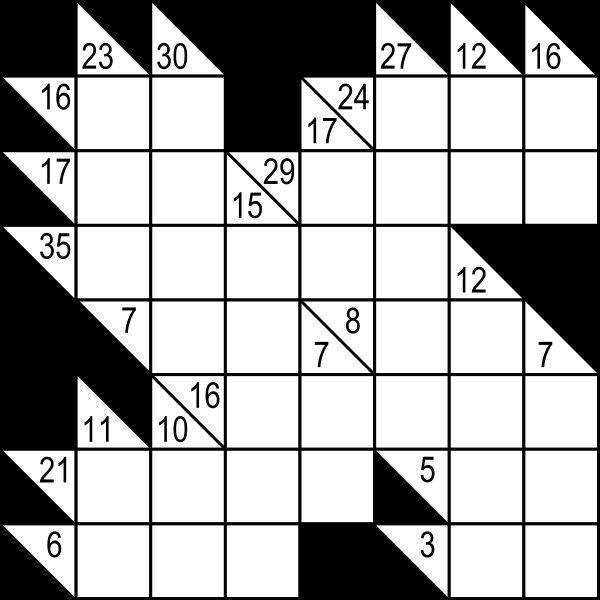
\includegraphics[scale=0.5]{kakuro} 
				\end{columns}
			\end{frame}

			\begin{frame}
				\frametitle{Genetic Algorithms - Evolving the Population}
				\begin{itemize} [<+->]
					\item Selection $\rightarrow$ Selection of best {\it individual}s to evolve to improve the population.
					\item Crossover $\rightarrow$ Creation of new {\it individual}s by combining traits of current unidentical {\it individual}s  with a hope of a better {\it fitness} value expected.
					\item Mutation $\rightarrow$ Randomly modify partialy the genes of individuals.
					\item REPEAT!!! $\rightarrow$ From Evaluation again until a satisfying {\it fitness} value is obtained.
				\end{itemize} 
			\end{frame}

		\subsection{Kakuro Algorithm Implementation}
			\begin{frame}
				\frametitle{Kakuro Algorithm Idea}
				\includegraphics[scale=0.48]{KakuroImpl} 
			\end{frame}

		\subsection{Kakuro Implementation Problems}
			\begin{frame}
				\frametitle{Kakuro Implementation Problems}
				Before the implementation of the algorithm:
				\begin{itemize} [<+->]
					\item Studying the Generic Algorithm.
					\item Finding the Best Algorithm for Crossover.
					\item Finding the Best Algorithm for Mutation.
					\item Kakuro Puzzles Represents.
				\end{itemize}
			\end{frame}

			\begin{frame}
				\frametitle{Kakuro Implementation Problems}
				During the implementation of the algorithm:
				\begin{itemize}
					\item There is an imprecision in float value division:
					\item $\rightarrow$ Ex: 1.7/10 = \underline{0.16999999999999998} !!
					\item The algorithm does not improve solutions:
					\item $\rightarrow$ Ex: Fitness value remains constantly at "5.25".
					\item Ignoring the value of performing unit testing and component testing, which causes misunderstanding with the fitness value

				\end{itemize}
			\end{frame}

		\subsection{Kakuro Solutions}
			\begin{frame}
				\frametitle{Suggested Solutions for Kakuro Problems}
				\begin{itemize} [<+->]
					\item Increase a Population Size.
					\item During a mutation of individuals, permutate sets of solutions to find the best set which leads to  the best fitness value.
				\end{itemize}
			\end{frame}


	\begin{frame}
		\frametitle{Programming Exercises - Final Presentation}
		\begin{center}
			Thank you!
		\end{center}
	\end{frame}

\end{document}